\documentclass{article}

\usepackage{amsmath}
\usepackage{tikz}
\usepackage{palatino}

\newcommand{\cset}{\mathbf{Set}}
\newcommand{\cposet}{\mathbf{Poset}}

\begin{document}
\begin{enumerate}
\item[1.9.10.1]
  The goal is to show that the limit of the two object diagram with arrows $f: A \rightarrow B$ and $g : A \rightarrow B$ is an equalizer of $f$ and $g$.
  \begin{center}
    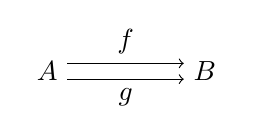
\begin{tikzpicture}
      \node (1) {$A$};
      \node [right of=1,xshift=1cm] (2) {$B$};

      \draw[transform canvas={yshift=0.1cm},->] (1) -- node[above] {$f$} (2);
      \draw[transform canvas={yshift=-0.1cm},->] (1) -- node[below] {$g$} (2);
    \end{tikzpicture}
  \end{center}
  To begin, a cone for this diagram consists of an object $X$ and arrows $a : X \rightarrow A$ and $b : X \rightarrow B$ such that the diagram commutes.
  \begin{center}
    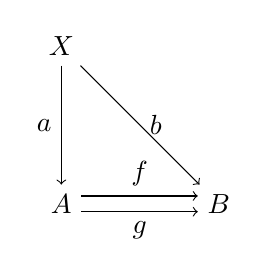
\begin{tikzpicture}
      \node (1) {$A$};
      \node [right of=1,xshift=1cm] (2) {$B$};
      \node [above of=1,yshift=1cm] (3) {$X$};

      \draw[transform canvas={yshift=0.1cm},->] (1) -- node[above] {$f$} (2);
      \draw[transform canvas={yshift=-0.1cm},->] (1) -- node[below] {$g$} (2);
      \draw[->] (3) -- node[left] {$a$} (1);
      \draw[->] (3) -- node[right] {$b$} (2);
    \end{tikzpicture}
  \end{center}
  However, $b$ is uniquely determined by the commutativity of the diagram to be the common composition $f \circ a = g \circ a$.
  (This is the same argument Pierce uses in his example of pullbacks as the limit of L-shaped diagrams.)

  \hfill{}
    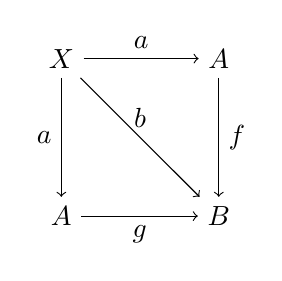
\begin{tikzpicture}
      \node (1) {$X$};
      \node [right of=1,xshift=1cm] (2) {$A$};
      \node [below of=1,yshift=-1cm] (3) {$A$};
      \node [right of=3,xshift=1cm] (4) {$B$};

      \draw[->] (2) -- node[right] {$f$} (4);
      \draw[->] (3) -- node[below] {$g$} (4);
      \draw[->] (1) -- node[above] {$a$} (2);
      \draw[->] (1) -- node[left] {$a$} (3);
      \draw[->] (1) -- node[above] {$b$} (4);
    \end{tikzpicture}
  \hfill{}
    \begin{tikzpicture}
      \node (1) {$X$};
      \node [right of=1,xshift=1cm] (2) {$A$};
      \node [below of=1,yshift=-1cm] (3) {$A$};
      \node [right of=3,xshift=1cm] (4) {$B$};

      \draw[->] (2) -- node[right] {$f$} (4);
      \draw[->] (3) -- node[below] {$g$} (4);
      \draw[->] (1) -- node[above] {$a$} (2);
      \draw[->] (1) -- node[left] {$a$} (3);
      %% \draw[->] (1) -- node[right] {$b$} (4);
    \end{tikzpicture}
  \hfill{}
  
  A limit of these diagrams has the property that any other $X'$ with an arrow $a'$ making the diagram commute has a unique arrow $k : X' \rightarrow X$.
  This gives us a commutative diagram identical to the equalizer diagram.
  Therefore our limit is an equalizer of $f$ and $g$.
  \begin{center}
    \begin{tikzpicture}
      \node (1) {$X$};
      \node[below of=1,yshift=-1cm] (2) {$X'$};
      \node [right of=1,xshift=1cm] (3) {$A$};
      \node [right of=3,xshift=1cm]  (4) {$B$};

      \draw[->] (1) -- node[above] {$a$} (3);
      \draw[dashed,->] (2) -- node[left] {$k$} (1);
      \draw[->] (2) -- node[below] {$a'$} (3);
      \draw[transform canvas={yshift=0.1cm},->] (3) -- node[above] {$f$} (4);
      \draw[transform canvas={yshift=-0.1cm},->] (3) -- node[below] {$g$} (4);
    \end{tikzpicture}
  \end{center}
  
\newpage
\item[1.9.10.2]
  The limit is the infinium $i\in \mathcal{C}$
  of the elements $D_i\in \mathcal{D}$.

  The colimit is the suprenam in $\mathcal{C}$ of
  the same elements, $D_i \in \mathcal{D}$.

\item[]
\item[1.9.10.3]
  We can construct limits of arbitrary diagrams $D$ in $\cset$ or $\cposet$ by taking as limit the product object $\prod D_i$ of all objects in the diagram.
  Firstly, the object $\prod D_i$ exists because $\cset$ and $\cposet$ are categories with products.
  Commutativity of all mediating triangles $f_{ij} \circ \pi_i = \pi_j$ follows because all arrows $f_{ij}$ in $\cset$ and $\cposet$ are total maps.
  Uniqueness of the limit $\prod D_i$ comes from the universal property of product objects.
  \begin{center}
    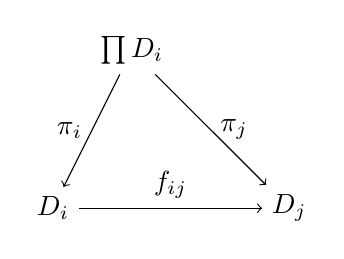
\begin{tikzpicture}
      \node (1) {$\prod D_i$};
      \node[below of=1,xshift=-1cm,yshift=-1cm] (2) {$D_i$};
      \node[right of=2,xshift=2cm] (3) {$D_j$};

      \draw[->] (1) -- node[left] {$\pi_i$} (2);
      \draw[->] (1) -- node[right] {$\pi_j$} (3);
      \draw[->] (2) -- node[above] {$f_{ij}$} (3);
    \end{tikzpicture}
  \end{center}

\item[]
\item[1.9.10.4]
  Dually, colimits in $\cset$ and $\cposet$ are the coproduct of all objects in the diagram.
  Again, the coproduct always exists because $\cset$ and $\cposet$ are categories with products, the mediating triangles commute because the arrows in these categories are total maps, and uniqueness follows from the universal property of coproducts.

  Going further, we can dualize the limit theorem by using coproducts and coequalizers.
  Construct the coproduct $\sum D_i$ of all objects in the diagram and the coproduct $\sum e$ of all edge destinations.
  The colimit is the codomain of the coequalizer of the unique arrows from $\sum e$ to $\sum D_i$.
  
\end{enumerate}
\end{document}
